\newcommand{\tr}{\textsc{Tree Reconstruction}\xspace}
\newcommand{\tc}{\textsc{3COL}\xspace}

\section*{Problem 4}

{\bf Reduction from \tc to \tr}

We will describe a reduction from \tc to \tr. For this reduction we
will define gadgets for every vertex and edge in the input \tc graph
$G$, by creating one tree for every vertex and one tree for every
edge, which are described by Figure \ref{q4:vertextree}
and Figure \ref{q4:edgetree}.
In addition we will create a single scaffolding tree, which is
described by Figure \ref{q4:scafftree}. Finally, in this
reduction we will set the value of $m$ to be $H + 4n + 4$,
where $n$ is the number vertices in $G$, and $H$ corresponds
to the constant appearing in the tree gadgets, which is assumed
to be very large (greater than $4n + 4$).

This reduction is clearly polynomial time because the size of
each tree is linear in $n$, and the number of trees is at worst
quadratic in $n$. In order to prove that this reduction is correct,
we need to argue that a graph $G$ is 3-colorable if and only if there
is a tree $T$ with at most $m$ vertices that has all the gadget trees
as subtrees.\\ 
\\
{\bf Forward direction of proof of reduction correctness}\\
\\
For the forward direction, suppose $G$ is 3-colorable. We will
describe how to create a tree $T$ of size $m$ with all the gadget
trees as subtrees. First we initialize $T$ as the scaffolding
tree $T_S$, and we arbitrarily label the colors in a 3-coloring
of $G$ as $R$, $G$, and $B$. Now we will extend this tree
by adding a new node for every vertex $v_i$. Let $c = \text{color}(v_i)$.
We will create a new node $c_i$ and
add an edge from $v_i^c$ to $c_i$.

Now we argue that this $T$ has the desired properties.
We will refer to $\{h_1,\ldots,h_H\}$ along with $A$
as the ``hat'' of the tree, and $\{v_1^c,\ldots,v_n^c\}$ along
with $s^c$ as the ``$c$-stem'' of the tree (for $c \in \{R, G, B\}$).
First of all, $T_S$ had $H + 3n + 4$ nodes, and we 
added $n$ nodes to it to construct $T$, so clearly $T$
has exactly $m$ vertices.
Secondly, for each vertex $v_i$ in $G$ we attached a new node to
$v_i^c$ in $T_S$, where $c = \text{color}(v_i)$.
Thus the subtree of $T$ induced by the hat, the $c$-stem
of the tree, and $c_i$ is isomorphic to the vertex gadget
of $v_i$. Thirdly, for every edge $(v_i, v_j)$ we know
that $v_i$ and $v_j$ have different colors in $G$, so
the $c_i$ and $c_j$ nodes must have been added in different
branches of $G$. Thus the subtree induced by the hat,
the $\text{color}(v_i)$- and $\text{color}(v_j)$-stems of the
tree, $c_i$, and $c_j$ is isomorphic to the corresponding
edge gadget. Finally $T$ was constructed by extending $T_S$,
so $T_S$ is a subtree. Thus we have proved the forward
direction.\\
\\
{\bf Backwards direction of proof of reduction correctness}\\
\\
For the backwards direction of the proof, suppose we can
construct a tree $T$ with at most $m$ vertices containing
$T_S$ along with all the vertex and edge gadgets based on
$G$ as subtrees. We will argue from this that $G$ is 3-colorable.
First of all given that $T_S$ is a subtree, $T$ must have at least
$H + 3n + 4$ vertices, so it can have at most $n$ vertices
in addition to the vertices in the subtree isomorphic to $T_S$.
Now we will consider the possible ways that $T_S$ could be
extended to $T$ in order to incorporate the vertex and
edge gadgets. Since $H$ is so large, the hats of the gadget
subtrees must be the same as the hat of $T_S$ (else we would
have to add too many vertices; $T$ is a tree so any two nodes
can have at most one neighbor in common, so if there
were two vertices of degree $H + 1$ we would have more
than $m$ vertices in total).
Each vertex gadget $v_i$ requires
a path of length $n + 1$ prefixed by $A$, with an extra vertex
attached to the $(i+1)$'th node in the path. Obviously the
only way to satisfy this for all $n$ gadgets simultaneously,
given we can only add $n$ extra nodes,
would be to attach a new node to exactly one
of the three $v_i^{color}$ vertices for each
$i \in \{1,\ldots,n\}$. Therefore we can conclude that $T$
must be isomorphic to $T_S$ with $n$ such extra vertices attached.

Given we know the structure that $T$ must have,
we will argue how to 3-color $G$ based on $T$. First we
locate the vertex of maximum degree and label it as $A$,
and label its leaf neighbors as $\{h_1,\ldots,h_H\}$
arbitrarily. Then we arbitrarily label the three branches
corresponding to the remaining three children of $A$ as
$R$, $G$, and $B$, and label the depth-$i$ non-leaf nodes
in each branch as $v_i^R$, $v_i^G$, and $v_i^B$
respectively. Finally we arbitrarily label
one of the leaf node(s) at depth $i + 1$
in each branch as $s^R$, $s^G$, and $s^B$ respectively,
and for each $i$ we label the remaining unlabeled leaf node,
which must be attached to one of the $v_i^{color}$ nodes, as $c_i$.
Given what we have reasoned about
the structure of $T$ this is possible to do unambiguously (up
the choices flagged as arbitrary), and for
each $i$ exactly one of $v_i^R$, $v_i^G$, or $v_i^B$
will have a $c_i$ neighbor. We color each $v_i$ in $G$
according to the label of the branch that $c_i$ is in (either
$R$, $G$, or $B$).

To complete the backwards direction of the proof, we
will argue that this satisfies the constraint that neighboring
vertices in $G$ must have different colors. Suppose $(v_i, v_j) \in E(G)$.
Then given that the corresponding edge gadget is a subtree of $T$
it must be the case that there are degree-3 $v_i^{color}$
and $v_j^{color}$ nodes in separate
branches of $T$. This implies that $c_i$ and $c_j$ must be in separate
branches, so $v_i$ and $v_j$ will have been assigned different colors.
Therefore this 3-coloring is clearly valid, so $G$ is 3-colorable.\\
\\
{\bf Proof that \tr is in NP}\\
\\
Now we have established that \tc reduces to \tr, which implies
that \tr is in NP-HARD. All that remains in order to show that it is
in NP-COMPLETE is to prove that it is in NP. To see this we will
describe a polynomial-time verifier for ``yes'' instances of \tr.
The input string to the verifier will consist
of a reconstructed tree $T$ of
size at most $m$, along with isomorphism functions $\pi_i$ mapping every
node in each subtree $T_i$ to a node in $T$. Clearly this string
can be polynomial in length, as in the worst case the size of
an allowable $T$ is bounded above by the sum of all the subtree sizes,
and the size of each $\pi_i$ is at worst a constant multiple
of the size of each subtree. The verifier works by first counting
the number of nodes in $T$ to assert that it is less than $m$,
running DFS to assert that $T$ is in fact a tree, asserting that
each $\pi_i$ is a one-to-one function from $V(T_i)$ to $V(T)$,
and finally asserting that each $T_i$ is a subtree of $T$ one by one,
by asserting for every $(u, v) \in E(T_i)$ that
$(\pi_i(u), \pi_i(v)) \in E(T)$. This clearly runs in polynomial time, 
asserts that $T$ is a valid solution to the problem, and
cannot be fooled, as required.



\begin{figure}
\begin{tikzpicture}
  \node[shape=circle,draw=black] (A) at (0,0) {A};
  \node[shape=circle,draw=black] (h1) at (-1.5,2) {$h_0$};
  \node[shape=circle,draw=black] (h2) at (-0.5,2) {$h_1$};
  \node (dots) at (0.5,2) {$\ldots$};
  \node[shape=circle,draw=black] (hH) at (1.5,2) {$h_H$};
  \node[shape=circle,draw=black] (v1) at (0,-2) {$v_1$};
  \node[shape=circle,draw=black] (v2) at (0,-4) {$v_2$};
  \node (dots1) at (0,-5) {$\ldots$};
  \node[shape=circle,draw=black] (vi) at (0,-6) {$v_i$};
  \node[shape=circle,draw=black] (ci) at (2,-6) {$c_i$};
  \node (dots2) at (0,-7) {$\ldots$};
  \node[shape=circle,draw=black] (vn) at (0,-8) {$v_n$};
  \node[shape=circle,draw=black] (s) at (0,-10) {$s$};
  \path (A) edge node {} (h1);
  \path (A) edge node {} (h2);
  \path (A) edge node {} (hH);
  \path (A) edge node {} (v1);
  \path (v1) edge node {} (v2);
  \path (v2) edge node {} (dots1);
  \path (dots1) edge node {} (vi);
  \path (vi) edge node {} (ci);
  \path (vi) edge node {} (dots2);
  \path (dots2) edge node {} (vn);
  \path (vn) edge node {} (s);
\end{tikzpicture}
\caption{Vertex gadget tree $T_{v_i}$ in \tr reduction for vertex $v_i$.
         This tree contains $H + n + 3$ vertices.}
\label{q4:vertextree}
\end{figure}

\begin{figure}
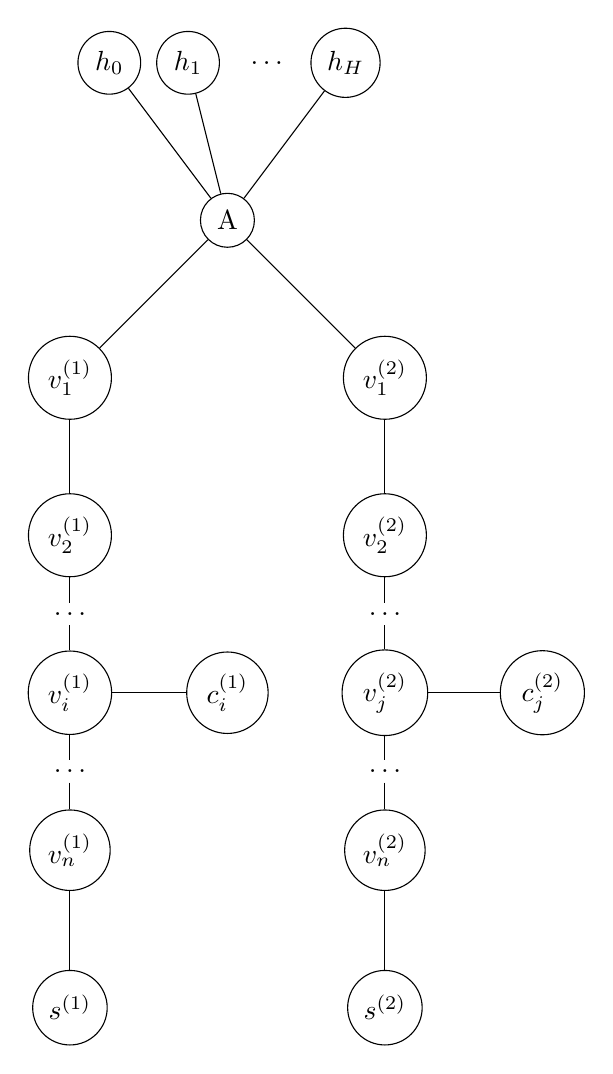
\begin{tikzpicture}
  \node[shape=circle,draw=black] (A) at (0,0) {A};
  \node[shape=circle,draw=black] (h1) at (-1.5,2) {$h_0$};
  \node[shape=circle,draw=black] (h2) at (-0.5,2) {$h_1$};
  \node (dots) at (0.5,2) {$\ldots$};
  \node[shape=circle,draw=black] (hH) at (1.5,2) {$h_H$};
  \node[shape=circle,draw=black] (v11) at (-2,-2) {$v_1^{(1)}$};
  \node[shape=circle,draw=black] (v12) at (2,-2) {$v_1^{(2)}$};
  \node[shape=circle,draw=black] (v21) at (-2,-4) {$v_2^{(1)}$};
  \node[shape=circle,draw=black] (v22) at (2,-4) {$v_2^{(2)}$};
  \node (dots1) at (-2,-5) {$\ldots$};
  \node (dots2) at (2,-5) {$\ldots$};
  \node[shape=circle,draw=black] (vi1) at (-2,-6) {$v_i^{(1)}$};
  \node[shape=circle,draw=black] (vj2) at (2,-6) {$v_j^{(2)}$};
  \node[shape=circle,draw=black] (ci1) at (0,-6) {$c_i^{(1)}$};
  \node[shape=circle,draw=black] (ci2) at (4,-6) {$c_j^{(2)}$};
  \node (dots3) at (-2,-7) {$\ldots$};
  \node (dots4) at (2,-7) {$\ldots$};
  \node[shape=circle,draw=black] (vn1) at (-2,-8) {$v_n^{(1)}$};
  \node[shape=circle,draw=black] (vn2) at (2,-8) {$v_n^{(2)}$};
  \node[shape=circle,draw=black] (s1) at (-2,-10) {$s^{(1)}$};
  \node[shape=circle,draw=black] (s2) at (2,-10) {$s^{(2)}$};
  \path (A) edge node {} (h1);
  \path (A) edge node {} (h2);
  \path (A) edge node {} (hH);
  \path (A) edge node {} (v11);
  \path (A) edge node {} (v12);
  \path (v11) edge node {} (v21);
  \path (v12) edge node {} (v22);
  \path (v21) edge node {} (dots1);
  \path (v22) edge node {} (dots2);
  \path (dots1) edge node {} (vi1);
  \path (dots2) edge node {} (vj2);
  \path (vi1) edge node {} (ci1);
  \path (vj2) edge node {} (ci2);
  \path (vi1) edge node {} (dots3);
  \path (vj2) edge node {} (dots4);
  \path (dots3) edge node {} (vn1);
  \path (dots4) edge node {} (vn2);
  \path (vn1) edge node {} (s1);
  \path (vn2) edge node {} (s2);
\end{tikzpicture}
\caption{Edge gadget tree $T_{(v_i,v_j)}$ in \tr reduction for edge $(v_i, v_j)$. This tree
         contains $H + 2n + 5$ vertices.}
\label{q4:edgetree}
\end{figure}


\begin{figure}
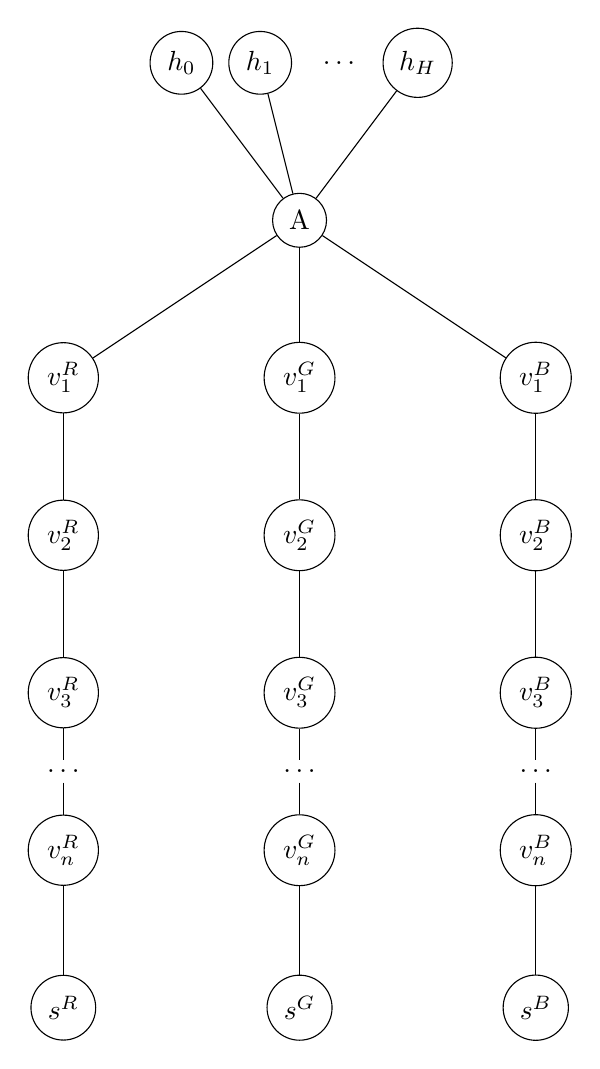
\begin{tikzpicture}
  \node[shape=circle,draw=black] (A) at (0,0) {A};
  \node[shape=circle,draw=black] (h1) at (-1.5,2) {$h_0$};
  \node[shape=circle,draw=black] (h2) at (-0.5,2) {$h_1$};
  \node (dots) at (0.5,2) {$\ldots$};
  \node[shape=circle,draw=black] (hH) at (1.5,2) {$h_H$};
  \node[shape=circle,draw=black] (v1R) at (-3,-2) {$v_1^R$};
  \node[shape=circle,draw=black] (v1G) at (0,-2) {$v_1^G$};
  \node[shape=circle,draw=black] (v1B) at (3,-2) {$v_1^B$};
  \node[shape=circle,draw=black] (v2R) at (-3,-4) {$v_2^R$};
  \node[shape=circle,draw=black] (v2G) at (0,-4) {$v_2^G$};
  \node[shape=circle,draw=black] (v2B) at (3,-4) {$v_2^B$};
  \node[shape=circle,draw=black] (v3R) at (-3,-6) {$v_3^R$};
  \node[shape=circle,draw=black] (v3G) at (0,-6) {$v_3^G$};
  \node[shape=circle,draw=black] (v3B) at (3,-6) {$v_3^B$};
  \node (dotsR) at (-3,-7) {$\ldots$};
  \node (dotsG) at (0,-7) {$\ldots$};
  \node (dotsB) at (3,-7) {$\ldots$};
  \node[shape=circle,draw=black] (vnR) at (-3,-8) {$v_n^R$};
  \node[shape=circle,draw=black] (vnG) at (0,-8) {$v_n^G$};
  \node[shape=circle,draw=black] (vnB) at (3,-8) {$v_n^B$};
  \node[shape=circle,draw=black] (sR) at (-3,-10) {$s^R$};
  \node[shape=circle,draw=black] (sG) at (0,-10) {$s^G$};
  \node[shape=circle,draw=black] (sB) at (3,-10) {$s^B$};
  \path (A) edge node {} (h1);
  \path (A) edge node {} (h2);
  \path (A) edge node {} (hH);
  \path (A) edge node {} (v1R);
  \path (A) edge node {} (v1G);
  \path (A) edge node {} (v1B);
  \path (v1R) edge node {} (v2R);
  \path (v1G) edge node {} (v2G);
  \path (v1B) edge node {} (v2B);
  \path (v2R) edge node {} (v3R);
  \path (v2G) edge node {} (v3G);
  \path (v2B) edge node {} (v3B);
  \path (v3R) edge node {} (dotsR);
  \path (v3G) edge node {} (dotsG);
  \path (v3B) edge node {} (dotsB);
  \path (dotsR) edge node {} (vnR);
  \path (dotsG) edge node {} (vnG);
  \path (dotsB) edge node {} (vnB);
  \path (vnR) edge node {} (sR);
  \path (vnG) edge node {} (sG);
  \path (vnB) edge node {} (sB);
\end{tikzpicture}
\caption{Scaffolding tree $T_S$ in \tr reduction. This tree contains $H + 3n + 4$ vertices.}
\label{q4:scafftree}
\end{figure}
